\section{Übung 11 – Entropie und Quellencodierung}

Diese Übung behandelt die Grundbegriffe der Informationstheorie und der
verlustlosen Quellencodierung: den \emph{Entscheidungsgehalt}
$H_0 = \log_2 N$ (Abschnitt~\ref{sec:informationsmass}), die \emph{Entropie}
$H = -\sum_i P(a_i)\log_2 P(a_i)$ (Abschnitt~\ref{sec:entropie-redundanz}),
die mittlere Codewortlänge $\mathrm{E}\{L\} = \sum_i l_i\,P(a_i)$ sowie die
\emph{Coderedundanz}

$$
r_c = \frac{\mathrm{E}\{L\} - H}{H}
$$

(Abschnitt~\ref{sec:quellencodierung}). Als Codierverfahren werden der
Fano-Code (Abschnitt~\ref{sec:shannon-fano}), der Huffman-Code
(Abschnitt~\ref{sec:huffman}) und die Lauflängencodierung
(Abschnitt~\ref{sec:laufllaengencodierung}) verwendet. Alle Logarithmen zur
Basis $2$ werden explizit angegeben; es gilt
$\log_2 x = \ln x / \ln 2$.

% ================================================================
\subsection*{Vorrechenaufgabe 11 – Verlustlose gemeinsame Quellencodierung}
% ================================================================

Eine Nachrichtenquelle sendet die drei Symbole $A$, $B$, $C$ mit gleicher
Wahrscheinlichkeit $P(A) = P(B) = P(C) = \tfrac{1}{3}$; aufeinanderfolgende
Symbole sind statistisch unabhängig.

% ---- a) --------------------------------------------------------
\subsubsection*{a) Entscheidungsgehalt eines Symbols}

\begin{beispiel}[Entscheidungsgehalt einer ternären Quelle]

\textbf{Gegeben:} Quelle mit $N = 3$ gleichwahrscheinlichen Symbolen.

\textbf{Gesucht:} Der Entscheidungsgehalt $H_0$ eines Symbols.

\textbf{Formel} (Entscheidungsgehalt, Abschnitt~\ref{sec:informationsmass}):

$$
H_0 = \log_2 N
$$

\textbf{Rechnung:}

$$
H_0 = \log_2 3 = \frac{\ln 3}{\ln 2} = \frac{1{,}0986}{0{,}6931} = 1{,}585\ \text{bit}.
$$

\textbf{Lösung:}

$$
\boxed{\;H_0 = \log_2 3 \approx 1{,}585\ \text{bit}.\;}
$$

Da die Symbole gleichwahrscheinlich sind, ist die Entropie gleich dem
Entscheidungsgehalt, $H = H_0 = 1{,}585$ bit; die Quelle selbst besitzt keine
Redundanz.

\end{beispiel}

% ---- b) --------------------------------------------------------
\subsubsection*{b) Fano-Code und Entscheidungsbaum}

\begin{beispiel}[Fano-Code für drei gleichwahrscheinliche Symbole]

\textbf{Gegeben:} $A,B,C$ mit je $P = \tfrac{1}{3}$.

\textbf{Gesucht:} Ein Fano-Code und der zugehörige Entscheidungsbaum.

\textbf{Formel} (Fano-Schema, Abschnitt~\ref{sec:shannon-fano}): sortieren nach
fallender Wahrscheinlichkeit, in zwei Gruppen möglichst gleicher
Summenwahrscheinlichkeit teilen, erste Gruppe mit $0$, zweite mit $1$
adressieren, rekursiv wiederholen.

\textbf{Rechnung:} Alle Symbole haben $\tfrac13$. Die günstigste Zweiteilung ist
$\{A\}$ (Wahrscheinlichkeit $\tfrac13$) gegen $\{B,C\}$ (Wahrscheinlichkeit
$\tfrac23$); Letztere wird nochmals in $\{B\}$ und $\{C\}$ geteilt:

\begin{center}
\begin{tabular}{c|c|cc|c}
Symbol & $P(a_i)$ & \multicolumn{2}{c|}{Code} & $l_i$ / bit \\
\hline
$A$ & $1/3$ & $0$ & $\times$ & $1$ \\
$B$ & $1/3$ & $1$ & $0$ & $2$ \\
$C$ & $1/3$ & $1$ & $1$ & $2$ \\
\end{tabular}
\end{center}

\textbf{Lösung:}

$$
\boxed{\;A \rightarrow 0, \qquad B \rightarrow 10, \qquad C \rightarrow 11.\;}
$$

\begin{center}
\begin{tikzpicture}[level distance=12mm,
  level 1/.style={sibling distance=28mm},
  level 2/.style={sibling distance=16mm},
  every node/.style={font=\small}]
\node[circle,draw,inner sep=1.5pt]{}
  child{node{$A$} edge from parent node[left]{$0$}}
  child{node[circle,draw,inner sep=1.5pt]{}
    child{node{$B$} edge from parent node[left]{$0$}}
    child{node{$C$} edge from parent node[right]{$1$}}
    edge from parent node[right]{$1$}};
\end{tikzpicture}
\end{center}

\end{beispiel}

% ---- c) --------------------------------------------------------
\subsubsection*{c) Mittlere Codewortlänge}

\begin{beispiel}[Mittlere Codewortlänge des ternären Fano-Codes]

\textbf{Gegeben:} Codewortlängen $l_A = 1$, $l_B = l_C = 2$ bit; $P = \tfrac13$.

\textbf{Gesucht:} Die mittlere Codewortlänge $\mathrm{E}\{L\}$.

\textbf{Formel} (Abschnitt~\ref{sec:quellencodierung}):
$\mathrm{E}\{L\} = \sum_i l_i\,P(a_i)$.

\textbf{Rechnung:}

$$
\mathrm{E}\{L\} = \frac13\cdot 1 + \frac13\cdot 2 + \frac13\cdot 2
= \frac{1+2+2}{3} = \frac{5}{3}\ \text{bit}.
$$

\textbf{Lösung:}

$$
\boxed{\;\mathrm{E}\{L\} = \tfrac{5}{3} \approx 1{,}667\ \text{bit/Symbol}.\;}
$$

\end{beispiel}

% ---- d) --------------------------------------------------------
\subsubsection*{d) Coderedundanz}

\begin{beispiel}[Coderedundanz des ternären Fano-Codes]

\textbf{Gegeben:} $\mathrm{E}\{L\} = \tfrac53$ bit, $H = \log_2 3 = 1{,}585$ bit.

\textbf{Gesucht:} Die Coderedundanz $r_c$.

\textbf{Formel} (Abschnitt~\ref{sec:quellencodierung}):
$r_c = \dfrac{\mathrm{E}\{L\} - H}{H}$.

\textbf{Rechnung:}

$$
r_c = \frac{\tfrac53 - 1{,}585}{1{,}585}
= \frac{1{,}667 - 1{,}585}{1{,}585}
= \frac{0{,}082}{1{,}585} = 0{,}0515.
$$

\textbf{Lösung:}

$$
\boxed{\;r_c = \frac{\tfrac53 - \log_2 3}{\log_2 3} \approx 0{,}0515
\mathrel{\widehat{=}} 5{,}15\,\%.\;}
$$

Der Einzelsymbol-Code verschwendet also gut $5\,\%$, weil die nicht ganzzahlige
Entropie $\log_2 3$ mit ganzzahligen Codewortlängen nicht exakt erreichbar ist.

\end{beispiel}

% ---- e) --------------------------------------------------------
\subsubsection*{e) Kartesische Produktmenge zweier Symbole}

\begin{beispiel}[Symbolpaare und ihre Auftrittswahrscheinlichkeiten]

\textbf{Gegeben:} Zwei aufeinanderfolgende, unabhängige Symbole aus
$\{A,B,C\}$.

\textbf{Gesucht:} Die kartesische Produktmenge und die
Auftrittswahrscheinlichkeiten der Paare.

\textbf{Formel:} Bei Unabhängigkeit ist $P(xy) = P(x)\,P(y)$.

\textbf{Rechnung / Lösung:} Die Produktmenge umfasst $3^2 = 9$ Paare, jedes mit

$$
P(xy) = \frac13\cdot\frac13 = \frac19 \approx 0{,}111.
$$

$$
\boxed{\;\{AA,\,AB,\,AC,\,BA,\,BB,\,BC,\,CA,\,CB,\,CC\},
\qquad P = \tfrac19\ \text{je Paar}.\;}
$$

\end{beispiel}

% ---- f) --------------------------------------------------------
\subsubsection*{f) Fano-Code für Symbolpaare}

\begin{beispiel}[Fano-Code der neun gleichwahrscheinlichen Paare]

\textbf{Gegeben:} $9$ Paare mit je $P = \tfrac19$.

\textbf{Gesucht:} Fano-Code, Entscheidungsbaum, mittlere Codewortlänge und
Coderedundanz.

\textbf{Formel:} Fano-Schema (Abschnitt~\ref{sec:shannon-fano});
$\mathrm{E}\{L\}$ und $r_c$ nach Abschnitt~\ref{sec:quellencodierung}.

\textbf{Rechnung:} Bei $9$ gleichwahrscheinlichen Symbolen wird bei jeder
Teilung so nah wie möglich an der Hälfte getrennt (z.\,B. $4$ gegen $5$
Elemente). Rekursiv ergeben sich $7$ Codeworte der Länge $3$ und $2$ Codeworte
der Länge $4$:

\begin{center}
\begin{tabular}{c|c|c|c}
Paar & Code & $l_i$ & Paar$\;\to\;$Code \\
\hline
$AA$ & $000$  & $3$ & $CA \to 110$ \\
$AB$ & $001$  & $3$ & $CB \to 1110$ \\
$AC$ & $010$  & $3$ & $CC \to 1111$ \\
$BA$ & $011$  & $3$ & \\
$BB$ & $100$  & $3$ & \\
$BC$ & $101$  & $3$ & \\
\end{tabular}
\end{center}

\begin{center}
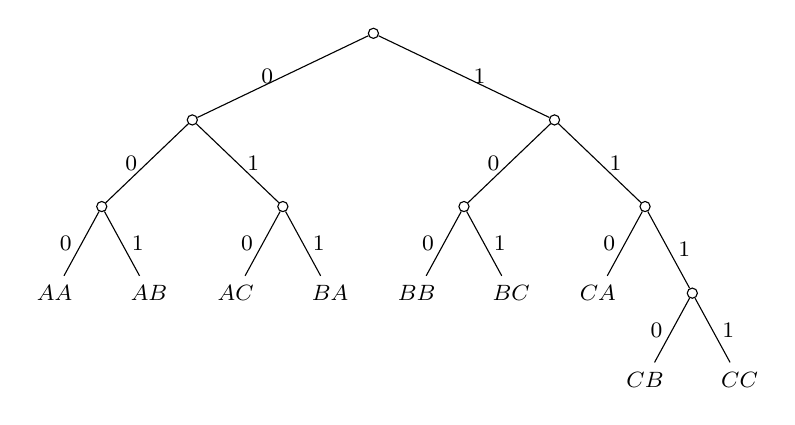
\begin{tikzpicture}[level distance=11mm,
  level 1/.style={sibling distance=46mm},
  level 2/.style={sibling distance=23mm},
  level 3/.style={sibling distance=12mm},
  level 4/.style={sibling distance=12mm},
  every node/.style={font=\footnotesize},
  dot/.style={circle,draw,inner sep=1.3pt}]
\node[dot]{}
 child{node[dot]{}
   child{node[dot]{}
     child{node{$AA$} edge from parent node[left]{$0$}}
     child{node{$AB$} edge from parent node[right]{$1$}}
     edge from parent node[left]{$0$}}
   child{node[dot]{}
     child{node{$AC$} edge from parent node[left]{$0$}}
     child{node{$BA$} edge from parent node[right]{$1$}}
     edge from parent node[right]{$1$}}
   edge from parent node[left]{$0$}}
 child{node[dot]{}
   child{node[dot]{}
     child{node{$BB$} edge from parent node[left]{$0$}}
     child{node{$BC$} edge from parent node[right]{$1$}}
     edge from parent node[left]{$0$}}
   child{node[dot]{}
     child{node{$CA$} edge from parent node[left]{$0$}}
     child{node[dot]{}
       child{node{$CB$} edge from parent node[left]{$0$}}
       child{node{$CC$} edge from parent node[right]{$1$}}
       edge from parent node[right]{$1$}}
     edge from parent node[right]{$1$}}
   edge from parent node[right]{$1$}};
\end{tikzpicture}
\end{center}

Mittlere Codewortlänge (je Paar, also je zwei Quellensymbole):

$$
\mathrm{E}\{L\} = \frac{7\cdot 3 + 2\cdot 4}{9} = \frac{29}{9}
\approx 3{,}222\ \text{bit/Paar} = 1{,}611\ \text{bit/Symbol}.
$$

Entropie eines Paares: $H = \log_2 9 = 2\log_2 3 = 3{,}170$ bit. Coderedundanz:

$$
r_c = \frac{\tfrac{29}{9} - \log_2 9}{\log_2 9}
= \frac{3{,}222 - 3{,}170}{3{,}170} = 0{,}0165.
$$

\textbf{Lösung:}

$$
\boxed{\;\mathrm{E}\{L\} = \tfrac{29}{9} \approx 3{,}222\ \text{bit/Paar}
\;(1{,}611\ \text{bit/Symbol}), \qquad r_c \approx 1{,}65\,\%.\;}
$$

Durch die gemeinsame Codierung von Paaren sinkt die Redundanz von $5{,}15\,\%$
(Einzelsymbol) auf $1{,}65\,\%$ -- die Codierung längerer Blöcke nähert sich der
Entropiegrenze an (Quellencodierungstheorem).

\end{beispiel}

% ================================================================
\subsection*{Aufgabe 11.1 – Quaternäre Quelle}
% ================================================================

\begin{beispiel}[Entscheidungsgehalt, Entscheidungsbaum und Code der quaternären Quelle]

\textbf{Gegeben:} Quelle mit $N = 4$ gleichwahrscheinlichen Symbolen
$A,B,C,D$, je $P = \tfrac14$.

\textbf{Gesucht:} a) Entscheidungsgehalt, b) binärer Entscheidungsbaum mit
minimaler Entscheidungszahl, c) binärer Code.

\textbf{Formel} (Entscheidungsgehalt, Abschnitt~\ref{sec:informationsmass}):
$H_0 = \log_2 N$.

\textbf{Rechnung:}

\emph{a)}
$$
H_0 = \log_2 4 = \log_2 2^2 = 2\ \text{bit}.
$$

\emph{b)} Da $H_0 = 2$ bit ganzzahlig ist, wird die Entropiegrenze mit einem
vollständig \emph{balancierten} Baum exakt erreicht: pro Symbol sind genau
$2$ Entscheidungen nötig. Ein unsymmetrischer Baum bräuchte im Mittel mehr als
$2$ Fragen und ist daher nicht optimal.

\emph{c)} Aus dem balancierten Baum folgt ein $2$-Bit-Festlängencode.

\textbf{Lösung:}

$$
\boxed{\;H_0 = 2\ \text{bit}; \qquad
A\to 00,\; B\to 01,\; C\to 10,\; D\to 11.\;}
$$

\begin{center}
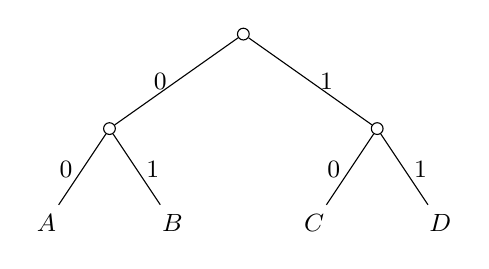
\begin{tikzpicture}[level distance=12mm,
  level 1/.style={sibling distance=34mm},
  level 2/.style={sibling distance=16mm},
  every node/.style={font=\small},
  dot/.style={circle,draw,inner sep=1.5pt}]
\node[dot]{}
 child{node[dot]{}
   child{node{$A$} edge from parent node[left]{$0$}}
   child{node{$B$} edge from parent node[right]{$1$}}
   edge from parent node[left]{$0$}}
 child{node[dot]{}
   child{node{$C$} edge from parent node[left]{$0$}}
   child{node{$D$} edge from parent node[right]{$1$}}
   edge from parent node[right]{$1$}};
\end{tikzpicture}
\end{center}

Mittlere Codewortlänge $\mathrm{E}\{L\} = 2$ bit $= H_0$; die Redundanz ist
$r_c = 0$.

\end{beispiel}

% ================================================================
\subsection*{Aufgabe 11.2 – Bildübertragung}
% ================================================================

\begin{beispiel}[Informationsmenge eines Grauwertbildes]

\textbf{Gegeben:} Grauwertbild mit $1024 \times 800$ Bildpunkten;
$N = 256$ gleichwahrscheinliche Graustufen; keine statistischen
Abhängigkeiten zwischen den Bildpunkten.

\textbf{Gesucht:} a) Informationsmenge pro Bildpunkt, b) Gesamt-Informationsmenge.

\textbf{Formel} (Abschnitt~\ref{sec:informationsmass}): $H_0 = \log_2 N$ pro
Bildpunkt; bei Unabhängigkeit addieren sich die Informationsmengen.

\textbf{Rechnung:}

\emph{a)}
$$
H_0 = \log_2 256 = \log_2 2^8 = 8\ \text{bit/Bildpunkt}.
$$

\emph{b)} Anzahl der Bildpunkte: $1024 \cdot 800 = 819\,200$. Bei Unabhängigkeit
ist die Gesamtinformation die Summe:

$$
I_{\text{ges}} = 819\,200 \cdot 8\ \text{bit} = 6\,553\,600\ \text{bit}
= 6{,}5536\ \text{Mbit} = 819\,200\ \text{Byte} = 800\ \text{KiB}.
$$

\textbf{Lösung:}

$$
\boxed{\;H_0 = 8\ \text{bit/Bildpunkt}, \qquad
I_{\text{ges}} = 6\,553\,600\ \text{bit} \approx 6{,}55\ \text{Mbit}.\;}
$$

Ohne Ausnutzung von Abhängigkeiten (Redundanz) benötigt das Bild volle
$8$ bit je Punkt -- reale Bilder lassen sich dank Nachbarschaftskorrelationen
deutlich stärker komprimieren.

\end{beispiel}

% ================================================================
\subsection*{Aufgabe 11.3 – Datenraten im Mobilfunk (GSM)}
% ================================================================

\begin{beispiel}[Zeitschlitze und Nutzdatenraten im GSM-System]

\textbf{Gegeben:} Pro Zeitschlitz werden $148$ bit übertragen, davon $114$ bit
Nutzinformation; ein Zeitschlitz dauert $T_{\text{S}} = 546{,}5\ \mu\text{s}$,
gefolgt von einer Sendepause $T_{\text{P}} = 30{,}5\ \mu\text{s}$.

\textbf{Gesucht:} a) Zeitschlitze pro Sekunde, b) maximale Nutzdatenrate $R$
(jeder $8$. Zeitschlitz, $24$ von $26$ für Nutzdaten), c) HSCSD-Rate $R'$
($2$ oder $3$ von $8$ Zeitschlitzen, $24$ von $26$).

\textbf{Formel:} Periodendauer je Zeitschlitz
$T = T_{\text{S}} + T_{\text{P}}$; Rate $=$ Bitzahl $/$ Zeit.

\textbf{Rechnung:}

\emph{a)} Ein Zeitschlitz belegt

$$
T = 546{,}5 + 30{,}5 = 577\ \mu\text{s},
$$

also

$$
n = \frac{1\ \text{s}}{577\ \mu\text{s}} = \frac{10^6}{577}
\approx 1733{,}1\ \frac{\text{Zeitschlitze}}{\text{s}}.
$$

(Kontrolle: $8$ Zeitschlitze bilden einen Rahmen von
$8\cdot 577\ \mu\text{s} = 4{,}615\ \text{ms}$.)

\emph{b)} Ein Teilnehmer erhält jeden $8$. Zeitschlitz; von $26$ gesendeten
Zeitschlitzen tragen $24$ Nutzdaten mit je $114$ bit:

$$
R = \underbrace{\frac{1733{,}1}{8}}_{216{,}64\ \text{Slots/s}}
\cdot \frac{24}{26}\cdot 114\ \text{bit}
\approx 22\,800\ \frac{\text{bit}}{\text{s}} = 22{,}8\ \text{kbit/s}.
$$

\emph{c)} Bei HSCSD werden $2$ bzw. $3$ Zeitschlitze pro Rahmen zugeteilt; die
Rate ist entsprechend das $2$- bzw. $3$-fache von $R$:

$$
R'_{2} = 2\cdot 22{,}8 = 45{,}6\ \text{kbit/s}, \qquad
R'_{3} = 3\cdot 22{,}8 = 68{,}4\ \text{kbit/s}.
$$

\textbf{Lösung:}

$$
\boxed{\;n \approx 1733\ \text{Slots/s}, \quad R \approx 22{,}8\ \text{kbit/s},
\quad R' = 45{,}6\ \text{bzw.}\ 68{,}4\ \text{kbit/s}.\;}
$$

Die Werte entsprechen den bekannten GSM-Kanälen (Vollratenkanal
$22{,}8$ kbit/s, HSCSD-Bündelung mehrerer Zeitschlitze).

\end{beispiel}

% ================================================================
\subsection*{Aufgabe 11.4 – Mittlerer Informationsgehalt}
% ================================================================

Eine binäre Quelle liefert unabhängige Symbole $0$ und $1$ mit
$P(0) = 0{,}4$ und $P(1) = 0{,}6$.

% ---- a) b) -----------------------------------------------------
\subsubsection*{a) \& b) Entscheidungsgehalt und Entropie pro Symbol}

\begin{beispiel}[Entscheidungsgehalt und Entropie einer binären Quelle]

\textbf{Gegeben:} Binäre Quelle, $P(0) = 0{,}4$, $P(1) = 0{,}6$.

\textbf{Gesucht:} a) Entscheidungsgehalt $H_0$, b) Entropie $H$ pro Symbol.

\textbf{Formel} (Abschnitt~\ref{sec:informationsmass} und
\ref{sec:entropie-redundanz}):
$H_0 = \log_2 N$, $\;H = -\sum_i P(a_i)\log_2 P(a_i)$.

\textbf{Rechnung:}

\emph{a)}
$$
H_0 = \log_2 2 = 1\ \text{bit/Symbol}.
$$

\emph{b)} Mit $\log_2 0{,}4 = -1{,}3219$ und $\log_2 0{,}6 = -0{,}7370$:

$$
H = -0{,}4\log_2 0{,}4 - 0{,}6\log_2 0{,}6
= 0{,}4\cdot 1{,}3219 + 0{,}6\cdot 0{,}7370
= 0{,}5288 + 0{,}4422 = 0{,}9710\ \text{bit}.
$$

\textbf{Lösung:}

$$
\boxed{\;H_0 = 1\ \text{bit/Symbol}, \qquad H \approx 0{,}971\ \text{bit/Symbol}.\;}
$$

Wegen der ungleichen Wahrscheinlichkeiten ist $H < H_0$; die Quelle besitzt eine
Redundanz $r_q = 1 - H/H_0 = 2{,}9\,\%$.

\end{beispiel}

% ---- c) --------------------------------------------------------
\subsubsection*{c) Kartesische Produktmenge dreier Symbole}

\begin{beispiel}[Symboltripel und ihre Wahrscheinlichkeiten]

\textbf{Gegeben:} Drei aufeinanderfolgende, unabhängige Symbole; $P(0)=0{,}4$,
$P(1)=0{,}6$.

\textbf{Gesucht:} Produktmenge und Auftrittswahrscheinlichkeiten der Tripel.

\textbf{Formel:} $P(xyz) = P(x)P(y)P(z)$.

\textbf{Rechnung / Lösung:} $2^3 = 8$ Tripel; die Wahrscheinlichkeit hängt nur
von der Anzahl der Einsen ab:

\begin{center}
\begin{tabular}{c|c|c}
Tripel & Wahrscheinlichkeit & Wert \\
\hline
$111$ & $0{,}6^3$ & $0{,}216$ \\
$110,\,101,\,011$ & $0{,}6^2\cdot 0{,}4$ & $0{,}144$ \\
$100,\,010,\,001$ & $0{,}6\cdot 0{,}4^2$ & $0{,}096$ \\
$000$ & $0{,}4^3$ & $0{,}064$ \\
\end{tabular}
\end{center}

$$
\boxed{\;\{000,001,010,011,100,101,110,111\};\quad
\textstyle\sum P = 0{,}064 + 3\cdot 0{,}096 + 3\cdot 0{,}144 + 0{,}216 = 1.\;}
$$

\end{beispiel}

% ---- d) e) -----------------------------------------------------
\subsubsection*{d) \& e) Fano-Code und Entscheidungsbaum der Tripel}

\begin{beispiel}[Fano-Code für drei aufeinanderfolgende Binärsymbole]

\textbf{Gegeben:} Die $8$ Tripel mit den Wahrscheinlichkeiten aus c).

\textbf{Gesucht:} Fano-Code und zugehöriger Entscheidungsbaum.

\textbf{Formel:} Fano-Schema (Abschnitt~\ref{sec:shannon-fano}).

\textbf{Rechnung:} Sortieren nach fallender Wahrscheinlichkeit und fortgesetztes
Halbieren der Summenwahrscheinlichkeit liefert:

\begin{center}
\begin{tabular}{c|c|cccc|c}
Tripel & $P$ & \multicolumn{4}{c|}{Code} & $l_i$ \\
\hline
$111$ & $0{,}216$ & $0$ & $0$ &   &   & $2$ \\
$110$ & $0{,}144$ & $0$ & $1$ & $0$ &   & $3$ \\
$101$ & $0{,}144$ & $0$ & $1$ & $1$ &   & $3$ \\
$011$ & $0{,}144$ & $1$ & $0$ & $0$ &   & $3$ \\
$100$ & $0{,}096$ & $1$ & $0$ & $1$ &   & $3$ \\
$010$ & $0{,}096$ & $1$ & $1$ & $0$ &   & $3$ \\
$001$ & $0{,}096$ & $1$ & $1$ & $1$ & $0$ & $4$ \\
$000$ & $0{,}064$ & $1$ & $1$ & $1$ & $1$ & $4$ \\
\end{tabular}
\end{center}

\textbf{Lösung (Entscheidungsbaum):}

\begin{center}
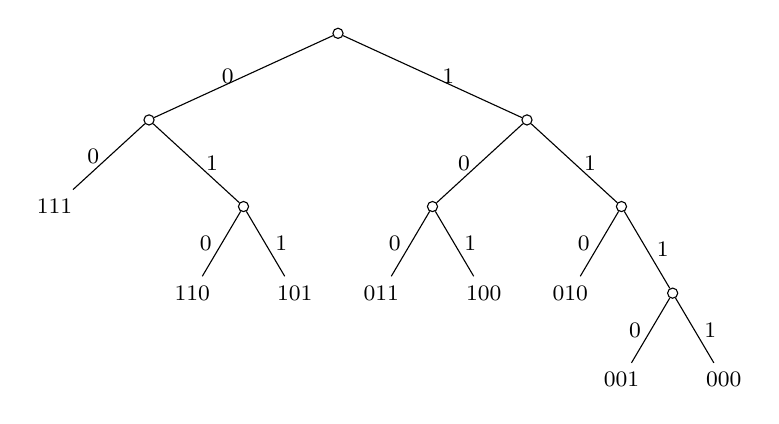
\begin{tikzpicture}[level distance=11mm,
  level 1/.style={sibling distance=48mm},
  level 2/.style={sibling distance=24mm},
  level 3/.style={sibling distance=13mm},
  level 4/.style={sibling distance=13mm},
  every node/.style={font=\footnotesize},
  dot/.style={circle,draw,inner sep=1.3pt}]
\node[dot]{}
 child{node[dot]{}
   child{node{$111$} edge from parent node[left]{$0$}}
   child{node[dot]{}
     child{node{$110$} edge from parent node[left]{$0$}}
     child{node{$101$} edge from parent node[right]{$1$}}
     edge from parent node[right]{$1$}}
   edge from parent node[left]{$0$}}
 child{node[dot]{}
   child{node[dot]{}
     child{node{$011$} edge from parent node[left]{$0$}}
     child{node{$100$} edge from parent node[right]{$1$}}
     edge from parent node[left]{$0$}}
   child{node[dot]{}
     child{node{$010$} edge from parent node[left]{$0$}}
     child{node[dot]{}
       child{node{$001$} edge from parent node[left]{$0$}}
       child{node{$000$} edge from parent node[right]{$1$}}
       edge from parent node[right]{$1$}}
     edge from parent node[right]{$1$}}
   edge from parent node[right]{$1$}};
\end{tikzpicture}
\end{center}

\end{beispiel}

% ---- f) --------------------------------------------------------
\subsubsection*{f) Coderedundanz}

\begin{beispiel}[Coderedundanz des Tripel-Fano-Codes]

\textbf{Gegeben:} Fano-Code aus d/e; Entropie pro Symbol $H = 0{,}971$ bit.

\textbf{Gesucht:} Die Coderedundanz $r_c$.

\textbf{Formel:} $\mathrm{E}\{L\} = \sum_i l_i P_i$;
$r_c = \dfrac{\mathrm{E}\{L\} - H_3}{H_3}$ mit $H_3 = 3H$.

\textbf{Rechnung:} Mittlere Codewortlänge je Tripel:

$$
\mathrm{E}\{L\} = 0{,}216\cdot 2 + (0{,}144\cdot 3 + 0{,}096\cdot 2 + 0{,}096)\cdots
$$
$$
\mathrm{E}\{L\} = 2\cdot 0{,}216 + 3\,(0{,}144\cdot 3 + 0{,}096\cdot 2)
+ 4\,(0{,}096 + 0{,}064) = 2{,}944\ \text{bit/Tripel}.
$$

Entropie eines Tripels: $H_3 = 3\cdot 0{,}971 = 2{,}913$ bit. Damit

$$
r_c = \frac{2{,}944 - 2{,}913}{2{,}913} = \frac{0{,}031}{2{,}913} = 0{,}0107.
$$

\textbf{Lösung:}

$$
\boxed{\;\mathrm{E}\{L\} = 2{,}944\ \text{bit/Tripel}\;(0{,}981\ \text{bit/Symbol}),
\qquad r_c \approx 1{,}07\,\%.\;}
$$

Gegenüber einem Einzelsymbol-Code ($\mathrm{E}\{L\} = 1$ bit,
$r_c = (1-0{,}971)/0{,}971 = 3{,}0\,\%$) reduziert die Blockcodierung von
Tripeln die Redundanz auf rund $1\,\%$.

\end{beispiel}

% ================================================================
\subsection*{Aufgabe 11.5 – Codierung unabhängiger Quellen}
% ================================================================

Zwei taktsynchrone, unabhängige Quellen: Quelle~1 sendet $1,2,3$ mit
$0{,}3;\,0{,}5;\,0{,}2$, Quelle~2 sendet $4,5,6$ mit $0{,}25;\,0{,}35;\,0{,}4$.

% ---- a) --------------------------------------------------------
\subsubsection*{a) Elementarereignisse je Quelle}

\begin{beispiel}[Elementarereignismengen der beiden Quellen]

\textbf{Gegeben / Gesucht:} Menge der Elementarereignisse je Quelle.

\textbf{Lösung:}

$$
\boxed{\;\Omega_1 = \{1,2,3\}, \qquad \Omega_2 = \{4,5,6\}.\;}
$$

\end{beispiel}

% ---- b) --------------------------------------------------------
\subsubsection*{b) Huffman-Codes und Redundanzen}

\begin{beispiel}[Huffman-Codierung der Einzelquellen]

\textbf{Gegeben:} $P_1(1,2,3) = (0{,}3;\,0{,}5;\,0{,}2)$,
$P_2(4,5,6) = (0{,}25;\,0{,}35;\,0{,}4)$.

\textbf{Gesucht:} Je ein Huffman-Code und die Coderedundanzen.

\textbf{Formel:} Huffman-Schema (Abschnitt~\ref{sec:huffman}); Entropie und
$r_c$ nach Abschnitt~\ref{sec:entropie-redundanz} bzw.
\ref{sec:quellencodierung}.

\textbf{Rechnung:} Für drei Symbole fasst Huffman stets die beiden kleinsten
Wahrscheinlichkeiten zusammen; das häufigste Symbol erhält $1$ bit, die beiden
übrigen $2$ bit.

\emph{Quelle 1} ($0{,}2 + 0{,}3 = 0{,}5$, dann mit $0{,}5$):

\begin{center}
\begin{tabular}{c|c|c|c}
Symbol & $P$ & Code & $l_i$ \\ \hline
$2$ & $0{,}5$ & $0$  & $1$ \\
$1$ & $0{,}3$ & $10$ & $2$ \\
$3$ & $0{,}2$ & $11$ & $2$ \\
\end{tabular}
\end{center}

$$
\mathrm{E}\{L_1\} = 0{,}5\cdot 1 + 0{,}3\cdot 2 + 0{,}2\cdot 2 = 1{,}5\ \text{bit}.
$$
$$
H_1 = -0{,}5\log_2 0{,}5 - 0{,}3\log_2 0{,}3 - 0{,}2\log_2 0{,}2 = 1{,}485\ \text{bit},
\quad
r_{c,1} = \frac{1{,}5 - 1{,}485}{1{,}485} = 0{,}98\,\%.
$$

\emph{Quelle 2} ($0{,}25 + 0{,}35 = 0{,}6$, dann mit $0{,}4$):

\begin{center}
\begin{tabular}{c|c|c|c}
Symbol & $P$ & Code & $l_i$ \\ \hline
$6$ & $0{,}4$  & $0$  & $1$ \\
$5$ & $0{,}35$ & $10$ & $2$ \\
$4$ & $0{,}25$ & $11$ & $2$ \\
\end{tabular}
\end{center}

$$
\mathrm{E}\{L_2\} = 0{,}4\cdot 1 + 0{,}35\cdot 2 + 0{,}25\cdot 2 = 1{,}6\ \text{bit}.
$$
$$
H_2 = 1{,}559\ \text{bit}, \qquad
r_{c,2} = \frac{1{,}6 - 1{,}559}{1{,}559} = 2{,}64\,\%.
$$

\textbf{Lösung:}

$$
\boxed{\;\mathrm{E}\{L_1\} = 1{,}5\ \text{bit},\ r_{c,1} \approx 0{,}98\,\%;
\qquad \mathrm{E}\{L_2\} = 1{,}6\ \text{bit},\ r_{c,2} \approx 2{,}64\,\%.\;}
$$

\end{beispiel}

% ---- c) --------------------------------------------------------
\subsubsection*{c) Gemeinsame Elementarereignisse}

\begin{beispiel}[Zweistellige Dezimalzahlen der Verbundquelle]

\textbf{Gegeben:} Quelle~1 erzeugt die höherwertige, Quelle~2 die
niederwertige Ziffer.

\textbf{Gesucht:} Menge aller gemeinsamen Elementarereignisse.

\textbf{Lösung:} Kartesisches Produkt $\Omega_1 \times \Omega_2$, $3\cdot 3 = 9$
Zahlen:

$$
\boxed{\;\{14,15,16,\;24,25,26,\;34,35,36\}.\;}
$$

\end{beispiel}

% ---- d) --------------------------------------------------------
\subsubsection*{d) Wahrscheinlichkeiten von „25`` und „34``}

\begin{beispiel}[Verbundwahrscheinlichkeiten zweier spezieller Zahlen]

\textbf{Gegeben:} Unabhängige Quellen; $P_1(2) = 0{,}5$, $P_2(5) = 0{,}35$,
$P_1(3) = 0{,}2$, $P_2(4) = 0{,}25$.

\textbf{Gesucht:} $P(\text{,,}25\text{``})$ und $P(\text{,,}34\text{``})$.

\textbf{Formel:} $P(xy) = P_1(x)\,P_2(y)$.

\textbf{Rechnung / Lösung:}

$$
P(25) = 0{,}5\cdot 0{,}35 = 0{,}175, \qquad
P(34) = 0{,}2\cdot 0{,}25 = 0{,}05.
$$

$$
\boxed{\;P(25) = 0{,}175, \qquad P(34) = 0{,}05.\;}
$$

\end{beispiel}

% ---- e) --------------------------------------------------------
\subsubsection*{e) Fano-Code der zweistelligen Zahlen}

\begin{beispiel}[Fano-Code der Verbundquelle]

\textbf{Gegeben:} Die $9$ Zahlen mit den Verbundwahrscheinlichkeiten
$P(xy) = P_1(x)P_2(y)$.

\textbf{Gesucht:} Ein Fano-Code.

\textbf{Formel:} Fano-Schema (Abschnitt~\ref{sec:shannon-fano}).

\textbf{Rechnung:} Nach fallender Wahrscheinlichkeit sortieren und rekursiv
halbieren (erste Teilung $\{26,25,24\}$ mit Summe $0{,}5$ gegen den Rest):

\begin{center}
\begin{tabular}{c|c|cccc|c}
Zahl & $P$ & \multicolumn{4}{c|}{Code} & $l_i$ \\
\hline
$26$ & $0{,}200$ & $0$ & $0$ &   &   & $2$ \\
$25$ & $0{,}175$ & $0$ & $1$ & $0$ &   & $3$ \\
$24$ & $0{,}125$ & $0$ & $1$ & $1$ &   & $3$ \\
$16$ & $0{,}120$ & $1$ & $0$ & $0$ &   & $3$ \\
$15$ & $0{,}105$ & $1$ & $0$ & $1$ &   & $3$ \\
$36$ & $0{,}080$ & $1$ & $1$ & $0$ & $0$ & $4$ \\
$14$ & $0{,}075$ & $1$ & $1$ & $0$ & $1$ & $4$ \\
$35$ & $0{,}070$ & $1$ & $1$ & $1$ & $0$ & $4$ \\
$34$ & $0{,}050$ & $1$ & $1$ & $1$ & $1$ & $4$ \\
\end{tabular}
\end{center}

Mittlere Codewortlänge (je zweistellige Zahl, also je zwei Quellensymbole):

$$
\mathrm{E}\{L\} = 0{,}2\cdot 2 + (0{,}175 + 0{,}125 + 0{,}12 + 0{,}105)\cdot 3
+ (0{,}08 + 0{,}075 + 0{,}07 + 0{,}05)\cdot 4 = 3{,}075\ \text{bit}.
$$

\textbf{Lösung:}

$$
\boxed{\;\mathrm{E}\{L\} = 3{,}075\ \text{bit/Zahl} = 1{,}5375\ \text{bit/Symbol}.\;}
$$

\end{beispiel}

% ---- f) --------------------------------------------------------
\subsubsection*{f) Vergleich: Zahlen- vs.\ Einzelziffern-Codierung}

\begin{beispiel}[Ist die gemeinsame Codierung günstiger?]

\textbf{Gegeben:} Einzelziffern-Codierung (Huffman) mit
$\mathrm{E}\{L_1\} + \mathrm{E}\{L_2\} = 1{,}5 + 1{,}6 = 3{,}1$ bit je
Symbolpaar; gemeinsame Fano-Codierung mit $3{,}075$ bit.

\textbf{Gesucht:} Ist die gemeinsame Codierung günstiger? Begründung.

\textbf{Rechnung:} Da die Quellen unabhängig sind, ist die Verbundentropie
$H = H_1 + H_2 = 1{,}485 + 1{,}559 = 3{,}044$ bit je Zahl. Vergleich der
mittleren Längen:

$$
\Delta = 3{,}1 - 3{,}075 = 0{,}025\ \text{bit je Symbolpaar}.
$$

\textbf{Lösung:}

$$
\boxed{\;3{,}075\ \text{bit} < 3{,}1\ \text{bit} \;\Rightarrow\;
\text{gemeinsame Codierung ist geringfügig günstiger.}\;}
$$

Der Vorteil ist klein, weil beide Quellen unabhängig sind und die
Einzel-Huffman-Codes bereits nahe am Optimum liegen. Der Fano-Code der Paare
kann jedoch die durch die \emph{nicht ganzzahligen} Idealcodewortlängen
entstehenden Rundungsverluste über zwei Symbole „mitteln`` und erreicht damit
$r_c = (3{,}075 - 3{,}044)/3{,}044 = 1{,}0\,\%$ statt der summierten
Einzelredundanz. Bei \emph{abhängigen} Quellen wäre der Gewinn deutlich größer.

\end{beispiel}

% ================================================================
\subsection*{Aufgabe 11.6 – Optimale Codierung eines Signals}
% ================================================================

Das zeitdiskrete Signal $s[k]$, $k = 1,\dots,20$, wird aus Bild~2
\emph{abgelesen} zu

$$
s[k] = \{2,3,3,1,0,-1,-1,-2,0,1,2,3,1,1,1,2,3,3,4,3\}.
$$

\begin{center}
\begin{tikzpicture}
\begin{axis}[
  width=13cm, height=6cm,
  xmin=0, xmax=21, ymin=-3, ymax=4.6,
  axis lines=middle,
  xlabel={$k$}, ylabel={$s[k]$},
  xtick={1,2,...,20}, ytick={-3,-2,...,4},
  tick label style={font=\scriptsize},
  ycomb, mark=*, mark size=1.4pt,
]
\addplot+[ycomb,black,mark=*] coordinates {
 (1,2)(2,3)(3,3)(4,1)(5,0)(6,-1)(7,-1)(8,-2)(9,0)(10,1)
 (11,2)(12,3)(13,1)(14,1)(15,1)(16,2)(17,3)(18,3)(19,4)(20,3)};
\end{axis}
\end{tikzpicture}
\end{center}

% ---- a) --------------------------------------------------------
\subsubsection*{a) Relative Häufigkeiten der Amplituden}

\begin{beispiel}[Relative Häufigkeiten des Signals]

\textbf{Gegeben:} Die $20$ abgelesenen Signalwerte $s[k]$.

\textbf{Gesucht:} Die relativen Häufigkeiten der Amplituden.

\textbf{Formel:} $h(a) = n(a)/20$.

\textbf{Rechnung / Lösung:} Auszählen der Werte ergibt

\begin{center}
\begin{tabular}{c|ccccccc}
Amplitude $a$ & $-2$ & $-1$ & $0$ & $1$ & $2$ & $3$ & $4$ \\
\hline
Anzahl $n(a)$ & $1$ & $2$ & $2$ & $5$ & $3$ & $6$ & $1$ \\
$h(a)$ & $0{,}05$ & $0{,}10$ & $0{,}10$ & $0{,}25$ & $0{,}15$ & $0{,}30$ & $0{,}05$ \\
\end{tabular}
\end{center}

$$
\boxed{\;h = (0{,}05;\,0{,}10;\,0{,}10;\,0{,}25;\,0{,}15;\,0{,}30;\,0{,}05),
\quad \textstyle\sum h = 1.\;}
$$

\end{beispiel}

% ---- b) --------------------------------------------------------
\subsubsection*{b) Huffman-Code für $s[k]$}

\begin{beispiel}[Huffman-Code des Signals mit Entscheidungsbaum]

\textbf{Gegeben:} Die relativen Häufigkeiten aus a).

\textbf{Gesucht:} Huffman-Entscheidungsbaum, Codetabelle und mittlere
Codewortlänge.

\textbf{Formel:} Huffman-Schema (Abschnitt~\ref{sec:huffman}),
$\mathrm{E}\{L\} = \sum_i l_i h_i$.

\textbf{Rechnung:} Wiederholtes Zusammenfassen der beiden kleinsten
Wahrscheinlichkeiten (in $20$-tel gerechnet:
$1,2,2,5,3,6,1$) liefert den folgenden Baum und die Codetabelle:

\begin{center}
\begin{tikzpicture}[level distance=10mm,
  level 1/.style={sibling distance=52mm},
  level 2/.style={sibling distance=26mm},
  level 3/.style={sibling distance=14mm},
  level 4/.style={sibling distance=13mm},
  every node/.style={font=\footnotesize},
  dot/.style={circle,draw,inner sep=1.3pt}]
\node[dot]{}
 child{node[dot]{}
   child{node[dot]{}
     child{node{$0$} edge from parent node[left]{$0$}}
     child{node{$-1$} edge from parent node[right]{$1$}}
     edge from parent node[left]{$0$}}
   child{node{$1$} edge from parent node[right]{$1$}}
   edge from parent node[left]{$0$}}
 child{node[dot]{}
   child{node[dot]{}
     child{node[dot]{}
       child{node{$-2$} edge from parent node[left]{$0$}}
       child{node{$4$} edge from parent node[right]{$1$}}
       edge from parent node[left]{$0$}}
     child{node{$2$} edge from parent node[right]{$1$}}
     edge from parent node[left]{$0$}}
   child{node{$3$} edge from parent node[right]{$1$}}
   edge from parent node[right]{$1$}};
\end{tikzpicture}
\end{center}

\begin{center}
\begin{tabular}{c|c|c|c}
Amplitude & $h$ & Code & $l_i$ \\ \hline
$3$  & $0{,}30$ & $11$   & $2$ \\
$1$  & $0{,}25$ & $01$   & $2$ \\
$2$  & $0{,}15$ & $101$  & $3$ \\
$0$  & $0{,}10$ & $000$  & $3$ \\
$-1$ & $0{,}10$ & $001$  & $3$ \\
$-2$ & $0{,}05$ & $1000$ & $4$ \\
$4$  & $0{,}05$ & $1001$ & $4$ \\
\end{tabular}
\end{center}

Mittlere Codewortlänge:

$$
\mathrm{E}\{L\} = (0{,}30 + 0{,}25)\cdot 2 + (0{,}15 + 0{,}10 + 0{,}10)\cdot 3
+ (0{,}05 + 0{,}05)\cdot 4 = 2{,}55\ \text{bit}.
$$

\textbf{Lösung:}

$$
\boxed{\;\mathrm{E}\{L\} = 2{,}55\ \text{bit/Symbol}.\;}
$$

Zum Vergleich: Entropie $H = 2{,}528$ bit, Entscheidungsgehalt
$H_0 = \log_2 7 = 2{,}807$ bit; die Coderedundanz beträgt nur
$r_c = (2{,}55 - 2{,}528)/2{,}528 = 0{,}86\,\%$.

\end{beispiel}

% ---- c) --------------------------------------------------------
\subsubsection*{c) Differenzsignal $d[k] = s[k] - s[k-1]$}

\begin{beispiel}[Differenzsignal der differentiellen Codierung]

\textbf{Gegeben:} $s[k]$ aus a); $s[0] = 0$; $d[k] = s[k] - s[k-1]$.

\textbf{Gesucht:} Das Differenzsignal $d[k]$ für $k = 1,\dots,20$.

\textbf{Rechnung / Lösung:} Gliedweise Differenzbildung ergibt

$$
d[k] = \{2,1,0,-2,-1,-1,0,-1,2,1,1,1,-2,0,0,1,1,0,1,-1\}.
$$

\begin{center}
\begin{tikzpicture}
\begin{axis}[
  width=13cm, height=6cm,
  xmin=0, xmax=21, ymin=-3, ymax=4.6,
  axis lines=middle,
  xlabel={$k$}, ylabel={$d[k]$},
  xtick={1,2,...,20}, ytick={-3,-2,...,4},
  tick label style={font=\scriptsize},
]
\addplot+[ycomb,black,mark=*,mark size=1.4pt] coordinates {
 (1,2)(2,1)(3,0)(4,-2)(5,-1)(6,-1)(7,0)(8,-1)(9,2)(10,1)
 (11,1)(12,1)(13,-2)(14,0)(15,0)(16,1)(17,1)(18,0)(19,1)(20,-1)};
\end{axis}
\end{tikzpicture}
\end{center}

\end{beispiel}

% ---- d) --------------------------------------------------------
\subsubsection*{d) Huffman-Code für das Differenzsignal}

\begin{beispiel}[Huffman-Code des Differenzsignals]

\textbf{Gegeben:} $d[k]$ aus c).

\textbf{Gesucht:} Huffman-Codetabelle und mittlere Codewortlänge.

\textbf{Formel:} Huffman-Schema (Abschnitt~\ref{sec:huffman}).

\textbf{Rechnung:} Relative Häufigkeiten der Differenzwerte:

\begin{center}
\begin{tabular}{c|ccccc}
Wert $d$ & $-2$ & $-1$ & $0$ & $1$ & $2$ \\
\hline
Anzahl & $2$ & $4$ & $5$ & $7$ & $2$ \\
$h(d)$ & $0{,}10$ & $0{,}20$ & $0{,}25$ & $0{,}35$ & $0{,}10$ \\
\end{tabular}
\end{center}

Huffman-Konstruktion ($0{,}10 + 0{,}10 = 0{,}20$, dann $0{,}20 + 0{,}20 = 0{,}40$
usw.):

\begin{center}
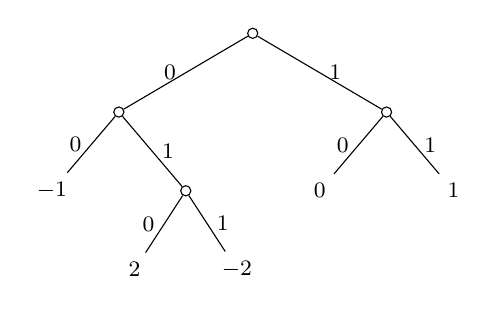
\begin{tikzpicture}[level distance=10mm,
  level 1/.style={sibling distance=34mm},
  level 2/.style={sibling distance=17mm},
  level 3/.style={sibling distance=13mm},
  every node/.style={font=\footnotesize},
  dot/.style={circle,draw,inner sep=1.3pt}]
\node[dot]{}
 child{node[dot]{}
   child{node{$-1$} edge from parent node[left]{$0$}}
   child{node[dot]{}
     child{node{$2$} edge from parent node[left]{$0$}}
     child{node{$-2$} edge from parent node[right]{$1$}}
     edge from parent node[right]{$1$}}
   edge from parent node[left]{$0$}}
 child{node[dot]{}
   child{node{$0$} edge from parent node[left]{$0$}}
   child{node{$1$} edge from parent node[right]{$1$}}
   edge from parent node[right]{$1$}};
\end{tikzpicture}
\end{center}

\begin{center}
\begin{tabular}{c|c|c|c}
Wert & $h$ & Code & $l_i$ \\ \hline
$1$  & $0{,}35$ & $11$  & $2$ \\
$0$  & $0{,}25$ & $10$  & $2$ \\
$-1$ & $0{,}20$ & $00$  & $2$ \\
$2$  & $0{,}10$ & $010$ & $3$ \\
$-2$ & $0{,}10$ & $011$ & $3$ \\
\end{tabular}
\end{center}

Mittlere Codewortlänge:

$$
\mathrm{E}\{L\} = (0{,}35 + 0{,}25 + 0{,}20)\cdot 2 + (0{,}10 + 0{,}10)\cdot 3
= 1{,}6 + 0{,}6 = 2{,}20\ \text{bit}.
$$

\textbf{Lösung:}

$$
\boxed{\;\mathrm{E}\{L\}_{d} = 2{,}20\ \text{bit/Symbol}
\;<\; \mathrm{E}\{L\}_{s} = 2{,}55\ \text{bit/Symbol}.\;}
$$

Die differentielle Codierung ist günstiger: das Differenzsignal konzentriert die
Wahrscheinlichkeitsmasse auf wenige kleine Werte (Ausnutzung der Korrelation
benachbarter Abtastwerte), wodurch die mittlere Codewortlänge um
$0{,}35$ bit/Symbol sinkt.

\end{beispiel}

% ================================================================
\subsection*{Aufgabe 11.7 – Bildcodierung}
% ================================================================

Das Schwarz-Weiß-Bild aus Bild~4 wird als Raster mit $8$ Zeilen und
$16$ Spalten ($128$ Bildpunkte) \emph{abgelesen}. Die folgende, aus der
Bildvorlage entnommene Anordnung dient als Grundlage aller Rechnungen
(schwarz $= 1$):

\begin{center}
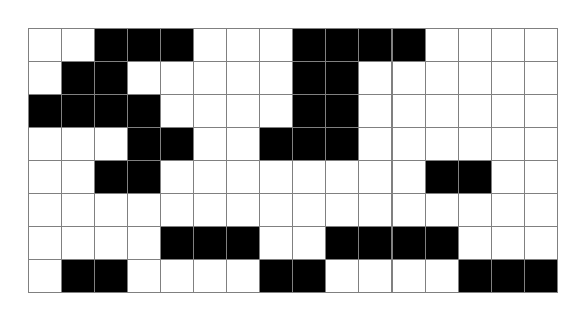
\begin{tikzpicture}[scale=0.42]
\fill[black] (2,7) rectangle (3,8);
\fill[black] (3,7) rectangle (4,8);
\fill[black] (4,7) rectangle (5,8);
\fill[black] (8,7) rectangle (9,8);
\fill[black] (9,7) rectangle (10,8);
\fill[black] (10,7) rectangle (11,8);
\fill[black] (11,7) rectangle (12,8);
\fill[black] (1,6) rectangle (2,7);
\fill[black] (2,6) rectangle (3,7);
\fill[black] (8,6) rectangle (9,7);
\fill[black] (9,6) rectangle (10,7);
\fill[black] (0,5) rectangle (1,6);
\fill[black] (1,5) rectangle (2,6);
\fill[black] (2,5) rectangle (3,6);
\fill[black] (3,5) rectangle (4,6);
\fill[black] (8,5) rectangle (9,6);
\fill[black] (9,5) rectangle (10,6);
\fill[black] (3,4) rectangle (4,5);
\fill[black] (4,4) rectangle (5,5);
\fill[black] (7,4) rectangle (8,5);
\fill[black] (8,4) rectangle (9,5);
\fill[black] (9,4) rectangle (10,5);
\fill[black] (2,3) rectangle (3,4);
\fill[black] (3,3) rectangle (4,4);
\fill[black] (12,3) rectangle (13,4);
\fill[black] (13,3) rectangle (14,4);
\fill[black] (4,1) rectangle (5,2);
\fill[black] (5,1) rectangle (6,2);
\fill[black] (6,1) rectangle (7,2);
\fill[black] (9,1) rectangle (10,2);
\fill[black] (10,1) rectangle (11,2);
\fill[black] (11,1) rectangle (12,2);
\fill[black] (12,1) rectangle (13,2);
\fill[black] (1,0) rectangle (2,1);
\fill[black] (2,0) rectangle (3,1);
\fill[black] (7,0) rectangle (8,1);
\fill[black] (8,0) rectangle (9,1);
\fill[black] (13,0) rectangle (14,1);
\fill[black] (14,0) rectangle (15,1);
\fill[black] (15,0) rectangle (16,1);
\draw[step=1,gray] (0,0) grid (16,8);
\end{tikzpicture}
\end{center}

% ---- a) --------------------------------------------------------
\subsubsection*{a) Relative Häufigkeiten Schwarz / Weiß}

\begin{beispiel}[Relative Häufigkeiten der Bildpunkte]

\textbf{Gegeben:} $128$ Bildpunkte; durch Auszählen ergeben sich $40$ schwarze
und $88$ weiße Punkte.

\textbf{Gesucht:} Relative Häufigkeiten.

\textbf{Formel:} $h = n/128$.

\textbf{Rechnung / Lösung:}

$$
\boxed{\;h_{\text{w}} = \frac{88}{128} = 0{,}6875, \qquad
h_{\text{s}} = \frac{40}{128} = 0{,}3125.\;}
$$

\end{beispiel}

% ---- b) --------------------------------------------------------
\subsubsection*{b) Mittlerer Informationsgehalt pro Bildpunkt}

\begin{beispiel}[Entropie eines Bildpunktes]

\textbf{Gegeben:} $P(\text{w}) = 0{,}6875$, $P(\text{s}) = 0{,}3125$.

\textbf{Gesucht:} Der mittlere Informationsgehalt $H$ pro Bildpunkt.

\textbf{Formel} (binäre Entropie, Abschnitt~\ref{sec:entropie-redundanz}):
$H = -P_{\text{w}}\log_2 P_{\text{w}} - P_{\text{s}}\log_2 P_{\text{s}}$.

\textbf{Rechnung:} Mit $\log_2 0{,}6875 = -0{,}5406$ und
$\log_2 0{,}3125 = -1{,}6781$:

$$
H = 0{,}6875\cdot 0{,}5406 + 0{,}3125\cdot 1{,}6781
= 0{,}3717 + 0{,}5244 = 0{,}896\ \text{bit}.
$$

\textbf{Lösung:}

$$
\boxed{\;H \approx 0{,}896\ \text{bit/Bildpunkt}.\;}
$$

Gegenüber $H_0 = 1$ bit/Bildpunkt (Festlängencodierung) liegt bereits hier ein
Kompressionspotenzial von rund $10\,\%$.

\end{beispiel}

% ---- c) --------------------------------------------------------
\subsubsection*{c) Relative Häufigkeiten der Lauflängen}

\begin{beispiel}[Lauflängenstatistik bei zeilenweiser Abtastung]

\textbf{Gegeben:} Zeilenweise Abtastung; jede Zeile beginnt mit einer weißen
Lauflänge (ggf.\ der Länge $0$); nach jeder Zeile folgt ein EOL-Symbol.

\textbf{Gesucht:} Relative Häufigkeiten der weißen und schwarzen Lauflängen
sowie die absolute Häufigkeit des EOL.

\textbf{Formel:} Lauflängencodierung (Abschnitt~\ref{sec:laufllaengencodierung}):
Zählung aufeinanderfolgender gleicher Bildpunkte.

\textbf{Rechnung / Lösung:} Auszählen der $8$ Zeilen ergibt $22$ weiße und
$15$ schwarze Lauflängen sowie $8$ EOL-Symbole:

\begin{center}
\begin{tabular}{c|ccccccccc}
weiße Länge & $0$ & $1$ & $2$ & $3$ & $4$ & $5$ & $6$ & $8$ & $16$ \\
\hline
Anzahl & $1$ & $2$ & $5$ & $3$ & $5$ & $1$ & $3$ & $1$ & $1$ \\
$h$ & \multicolumn{9}{c}{$\tfrac{1}{22},\tfrac{2}{22},\tfrac{5}{22},\tfrac{3}{22},\tfrac{5}{22},\tfrac{1}{22},\tfrac{3}{22},\tfrac{1}{22},\tfrac{1}{22}$} \\
\end{tabular}
\end{center}

\begin{center}
\begin{tabular}{c|ccc|c}
schwarze Länge & $2$ & $3$ & $4$ & EOL \\
\hline
Anzahl & $8$ & $4$ & $3$ & $8$ \\
\end{tabular}
\end{center}

Auf jede der $8$ Zeilen folgt genau ein EOL, also $\boxed{n_{\text{EOL}} = 8}$.
(Anmerkung: in diesem kleinen Ausschnitt treten auch schwarze Lauflängen der
Länge $2$--$4$ häufig auf; bei „schwarzer Schrift auf weißem Grund`` wären die
weißen Läufe im Mittel deutlich länger.)

\end{beispiel}

% ---- d) --------------------------------------------------------
\subsubsection*{d) Huffman-Code der weißen Lauflängen}

\begin{beispiel}[Huffman-Code für weiße Lauflängen]

\textbf{Gegeben:} Häufigkeiten der weißen Lauflängen aus c)
($22$ Läufe insgesamt).

\textbf{Gesucht:} Ein Huffman-Code.

\textbf{Formel:} Huffman-Schema (Abschnitt~\ref{sec:huffman}).

\textbf{Rechnung / Lösung:} Wiederholtes Zusammenfassen der beiden kleinsten
Häufigkeiten liefert die Codetabelle:

\begin{center}
\begin{tabular}{c|c|c|c}
weiße Länge & Anzahl & Code & $l_i$ \\ \hline
$2$  & $5$ & $00$    & $2$ \\
$4$  & $5$ & $01$    & $2$ \\
$3$  & $3$ & $101$   & $3$ \\
$6$  & $3$ & $110$   & $3$ \\
$1$  & $2$ & $1110$  & $4$ \\
$8$  & $1$ & $1000$  & $4$ \\
$16$ & $1$ & $1001$  & $4$ \\
$5$  & $1$ & $11110$ & $5$ \\
$0$  & $1$ & $11111$ & $5$ \\
\end{tabular}
\end{center}

$$
\boxed{\;\mathrm{E}\{L_{\text{w}}\}
= \frac{5\cdot 2 + 5\cdot 2 + 3\cdot 3 + 3\cdot 3 + 2\cdot 4 + 1\cdot 4
+ 1\cdot 4 + 1\cdot 5 + 1\cdot 5}{22}
= \frac{64}{22} \approx 2{,}91\ \text{bit/Lauf}.\;}
$$

\end{beispiel}

% ---- e) --------------------------------------------------------
\subsubsection*{e) Huffman-Code der schwarzen Lauflängen und des EOL}

\begin{beispiel}[Huffman-Code für schwarze Lauflängen und EOL]

\textbf{Gegeben:} Schwarze Lauflängen ($8\times 2$, $4\times 3$, $3\times 4$)
und $8$ EOL-Symbole; insgesamt $15 + 8 = 23$ Symbole.

\textbf{Gesucht:} Ein Huffman-Code.

\textbf{Formel:} Huffman-Schema (Abschnitt~\ref{sec:huffman}).

\textbf{Rechnung / Lösung:}

\begin{center}
\begin{tabular}{c|c|c|c}
Symbol & Anzahl & Code & $l_i$ \\ \hline
schwarz $2$ & $8$ & $11$   & $2$ \\
EOL         & $8$ & $0$    & $1$ \\
schwarz $3$ & $4$ & $101$  & $3$ \\
schwarz $4$ & $3$ & $100$  & $3$ \\
\end{tabular}
\end{center}

$$
\boxed{\;\mathrm{E}\{L_{\text{s+EOL}}\}
= \frac{8\cdot 2 + 8\cdot 1 + 4\cdot 3 + 3\cdot 3}{23}
= \frac{45}{23} \approx 1{,}96\ \text{bit/Symbol}.\;}
$$

\end{beispiel}

% ---- f) --------------------------------------------------------
\subsubsection*{f) Gesamt-Datenmenge}

\begin{beispiel}[Datenmenge des lauflängencodierten Bildes]

\textbf{Gegeben:} Die Huffman-Codes aus d) und e); Lauflängen und EOL aus c).

\textbf{Gesucht:} Die insgesamt anfallende Datenmenge.

\textbf{Formel:} Aufsummieren der Codewortlängen über alle Läufe und EOL-Symbole.

\textbf{Rechnung:}

\emph{Weiße Läufe:}
$$
5\cdot 2 + 5\cdot 2 + 3\cdot 3 + 3\cdot 3 + 2\cdot 4 + 1\cdot 4 + 1\cdot 4
+ 1\cdot 5 + 1\cdot 5 = 64\ \text{bit}.
$$

\emph{Schwarze Läufe:}
$$
8\cdot 2 + 4\cdot 3 + 3\cdot 3 = 16 + 12 + 9 = 37\ \text{bit}.
$$

\emph{EOL-Symbole:} $8\cdot 1 = 8$ bit.

$$
D_{\text{ges}} = 64 + 37 + 8 = 109\ \text{bit}.
$$

\textbf{Lösung:}

$$
\boxed{\;D_{\text{ges}} = 109\ \text{bit}
\;<\; 128\ \text{bit (unkodiert, 1 bit/Bildpunkt).}\;}
$$

Die Lauflängen- und Huffman-Codierung reduziert die Datenmenge von $128$ auf
$109$ bit, also um rund $15\,\%$. Der Gewinn stammt aus der Bündelung
gleichfarbiger Bildpunkte zu Läufen und der anschließenden Entropiecodierung;
bei realen, kontrastreichen Faksimile-Vorlagen mit langen weißen Läufen fällt
die Ersparnis noch erheblich größer aus.

\end{beispiel}
